\documentclass[a4paper,10pt]{scrartcl} % Die documentclass darf in keiner Latex-Datei fehlen, wenn die Datei allein ein Dokument erstellen soll. Es gibt allerdings die Möglichkeit andere Dateien, die Latex-Code enthalten in ein bestehendes Dokument einzubinden. Das geht mit "\include{anderesDokument}" oder "\input{andresDokument}" und ist besonders bei laaaaaaangen Dokumenten praktisch.
\usepackage[utf8]{inputenc}
\usepackage[german]{babel}
%\usepackage[T1]{fontenc}        % Erweiterte Textcodirung (z.B a" -> ä)
\usepackage{hyperref,url}       % Hyperlinks im pdf
\usepackage[all]{hypcap}        % Verhaltenskorrektur für hyperref
\usepackage{amssymb,amsmath}    % Schöne Formeln (AMS = American Mathematical Society)
\usepackage{graphicx}           % Bilder und Seitenränder
%\usepackage{natbib}		        % Bessere Bibliographie
%\bibliographystyle{dinat}       % Literaturverzeichnis nach DIN1505
%\usepackage{unicode-math}
\usepackage{cleveref}
\usepackage{caption}

\subject{Fortgeschrittenenpraktikum 1, Universit\"at Innsbruck}
\title{Diodenlaser}
\author{Gruppe T, Simon Hangl\footnote{\href{mailto:simon.hangl@uibk.ac.at}Simon.Hangl@uibk.ac.at}, Georg Zagler\footnote{\href{mailto:georg.zagler@student.uibk.ac.at}Georg.Zagler@student.uibk.ac.at}}
\date{Innsbruck, \today}

\begin{document}
\maketitle
\tableofcontents

\begin{abstract}
\textbf{Zusammenfassung}\\
In diesem Versuch wird eine Laserdiode untersucht. Dazu misst man den Diodenstrom und die Temperatur an der Diode um so die Anhängigkeit optischer Eigenschaften der Diode von diesen Grö\ss en zu bestimmen. Dabei findet man, dass ihre Leistung vom Diodenstrom abhängt, und die Frequenz mit steigendem Diodenstrom und steigender Temperatur sinkt.
\end{abstract}

\section{Einleitung}
\label{sec:Einleitung}
Laser werden seit ihrer Erfindung vor 30 Jahren in verschiedenen Bereichen der Forschung und Technik eingesetzt. Durch ihre hohe Intensität in Kombination mit ihrem engen Spektralbereich ermöglichen sie Anwendungen, welche mit herkömmlichen Strahlungsquellen nicht möglich sind. Während Laser in der physikalischen Forschung oft stationär betrieben werden und hohe Intensitäten und geringe Spektralbereiche aufweisen sollen, sind diese Eigenschaften in technischen Geräten meist zweitrangig. In Geräten wie CD-Spielern oder Laser-Pointern müssen Laser vor allem mobil sein, deshalb kommen dort Diodenlaser zum Einsatz. Diodenlaser sind, bei einer Grö\ss e vergleichbar mit einem Maiskorn, wesentlich kompakter als die Flaschen-gro\ss en, in der Forschung häufig verwendeten, HeNe-Laser. Jedoch besitzen Diodenlaser auch für viele spektroskopische Aufgaben ungünstige Eigenschaften, wie eine geringe Maximalleistung, geringe spektrale Reinheit, unsauberes Strahlprofil und keine kontinuierliche Verstimmbarkeit. In diesem Versuch sollen diese Eigenschaften untersucht werden.

\section{Grundlagen}
\label{sec:Grundlagen}
Für das Verständnis der Theorie und die Durchführung wurde die Anleitung zum Versuch \cite{Anleitung} verwendet.
Es gibt verschiedene Bauarten von Lasern, die mit verschiedenen $aktiven Medien$ betrieben werden; prinzipiell müssen zwei physikalische Vorgänge kombiniert werden, um einen Laser zu erzeugen:
\begin{itemize}
\item[i)] Ein aktives Medium (fest, flüsig oder gasförmig) muss vorliegen, in dem mehr Elektronen im angeregten Zustand sind, als im Grundzustand (Besetzungsinversion), sodass der Einfall von Photonen zu (erhöhter) stimulierter Emission führt.
\item[ii)] Ein Resonator, der sich vom aktiven Medium entfernende Photonen reflektiert.
\end{itemize}
Setzt man ein aktives Medium in Besetzungsinversion in einen Resonator, wird ausgehende spontane Emission an den Spiegeln des Resonators reflektiert und fürt im aktiven Medium zu stimulierter Emission. Wenn der Abstand der Spiegel des Resonators ein vielfaches der Hälfte der Wellenlänge der emittierten Photonen ist, so interferieren diese im Resonator konstruktiv. Mindestens ein Spiegel des Resonators muss eine Transmission $T \neq 0$ haben und die Leistung darf dadurch nicht abfallen.
\subsection{Resonator}
Ein optischer Resonator ist ein Aufbau aus mindestens zwei Spiegeln (oder reflektierenden Oberflächen) , die einen umlaufenden Lichstrahl in sich selbst zurückreflektieren. In einem Resonator werden Lichtstrahlen konstruktiv interferiert, welche $\lambda \cdot n / 2 = L$ erfüllen. $\lambda$ ist hier die Wellenlänge des Lichtstrahles, $n$ eine natürliche Zahl und $L$ die optische Weglänge bis der Lichtstrahl einmal den Resonator durchlaufen ist. Die optische Weglänge einer Distanz $s$ in einem Medium mit Brechzahl $n_B$ entspricht $L = n_B \cdot s$. Ein sehr einfacher Resonator ist das Fabry-Perot Interferometer, welches aus zwei gegenseitigen Spiegeln besteht. Er findet in unserem Versuch Anwendung. Der freie Spektralbereich $\Delta \nu$ zwischen zwei Moden eines Resonators ergibt sich aus $\Delta \nu = c/(2L)$. Die einzelnen Moden sind im Frequenz-Raum nicht scharf, sondern besitzen eine Breite, die von dem freien Spektralbereich und der Reflektivität $R$ der Spiegel abhängig ist.
\subsection{Diode}
In diesem Versuch bauen wir einen Diodenlaser. Das aktive Medium ist also eine Diode. Eine Diode besteht aus zwei dotierten Halbleitern, welche zusammengestellt werden. Dotierte Halbleiter bestehen aus einem Halbleiter-Kristall (z.B. Si oder Ge) in dem Framdatome eingebracht werden, welche nicht die gleiche Elektronenkonfiguration besitzen. Ein Halbleiter ist (n)-dotiert, besitzt also mehr Elektronen als der undotierte Halbleiter und damit auch Elektronen im Leitungsband (tiefstes nicht voll besetztes Band des undotierten Halbleiters). Ein Halbleiter ist (p)-dotiert, besitzt also weniger Elektronen als der undotierte Halbleiter und damit auch Löcher im Valenzband (höchstes voll besetztes Band des undotierten Halbleiters). An der Verbindungsfläche der beiden Halbleiter in der Diode rekombinieren die Elektronen des (n)- mit denen des (p)-dotierten Halbleiters, ein Elektron vom Leitungsband springt in ein Loch im Valenzband. Bei der Rekombination wird ein Photon mit der Energie $E = h \nu$ entsprechend der Energieabstände des Lochs und des Elektrons emittiert. Da die Dotierungs-Atome im (n)-Halbleiter als Kationen zurückbleiben, und im (p)-Halbleiter als Anionen, ergibt sich eine Drift-Spannung, welche der Diffusionsspannung der Elektronen und Löcher entgegengesetzt ist. Ohne extern angelegter Spannung bricht die Rekombination nach kurzer Zeit ab.\\


\begin{figure}
\centering
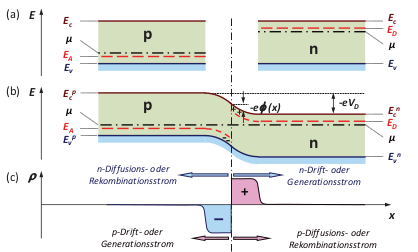
\includegraphics[width=0.7\textwidth]{Bilder/Halbleiter_2.png}
\caption{Bänder der bieden Dotierten Halbleiter. (a) (p)- und (n)-dotierte Halbleiter einzeln, $\mu$ beschreibt bis wo die Zustände mit Elektronen gefüllt sind (unterliegt einer Fermi-Vertielung, $\mu$ beschreibt die Kante bei Temperatur T = 0). Oben jeweils $E_C$: Leitungsband, unten $E_V$: Valenzband. Je nach dotierung werden diese leicht verschoben. (b) Verlauf der Bänder am p-n-Übergang im thermischen Gleichgewicht. (c) Verlauf der Raumladungszone $\rho (x)$ im Bereich des Überganges. Bild entnommen aus \cite{Marx}
}
\label{fig:Halbleiter}
\end{figure}
Legt man an der Diode eine Spannung an, sodass sie in Durchlassrichtung geschaltet ist, werden die Löcher im Valenzband und die Elektronen im Leitungsband in Richtung p-n-Übergang gedrückt, und eine Besetzungsinversion kommt zustande. Ein Photon das spontan emittiert wurde und durch die Spiegel reflektiert wird, löst in der Diode eine induzierte Emission aus. Das dabei emittierte Photon hat die gleiche Translationsrichtung, Wellenlänge und Phase wie das reflektierte Photon.\\
In unserem Versuch werden die Spiegel des Resonators an der Diode durch den Übergang vom Kristall in die Luft und dem damit verbundenen Brechzahl-Indexwechsel gebildet.\\
Im ersten Teil des Versuches werden der Schwellenstrom $I_{\text{th}}$(T), ab dem die Diode Laserstrahlen aussendet, und der Quanten-Wirkungsgrad $\eta$(T), also der Wirkungsgrad der Umwandlung von Strom-Quanten in Licht-Quanten, untersucht.Der Quanten-Wirkungsgrad ist gegeben durch
\begin{equation}
\label{eqn:Quanten_Winrkungsgrad}
\eta_{\text{Q}} = \frac{2e\lambda}{hc}\eta = \frac{2e}{E_{\text{photon}}}\eta
\end{equation}
wobei $e$ die Elementarladung und $E_{\text{Photon}} = hc/\lambda$ die Energie eines Photons mit Wellenlänge $\lambda$. Misst man die Leistung der Diode bei gleicher Temperatur und verschiedenem Strom, so erhält man aus der Steigung den Wirkungsquerschnitt $\eta$ der Diode und kann auf $\eta_{\text{Q}}$ schlie\ss en.

\section{Aufbau}
\label{sec:Aufbau}
Die Diode wird über eine regelbare Stromquelle betrieben, an welcher der regelbare Strom angezeigt wird. Sie steckt in einem Apparat (Laser Diode Mount with Integrated TEC and Controller \cite{Mount}), welcher zur Temperatur-Regulierung dient und mit welchem die Temperatur an der Diode im Bereich zwischen $20$ und $30^\circ{\text{C}}$ geändert kann. Das von der Diode ausgehende Licht wird mit einer Linse kollimiert. Im ersten Teil des Versuches, wird das Licht dahinter mit einer Linse auf eine Photodiode gebündelt. Die Leistung an der Photodiode wird mit einem Powermeter gemessen. Für den zweiten Teil des Versuches wird der Laserstrahl nach dem Kollimator mit zwei Spiegeln in ein Fabry-Perot-Interferometer gelenkt. Dieses besitzt einen variablen Spiegelabstand, der durch ein Piezo eingestellt werden kann. Ein Funktionsgenerator ist an einen Hochspannungsgenerator geschalten und versorgt das Piezo mit einem Dreieck-Signal. Am Ausgangsspiegel bündelt eine Linse den Strahl auf die Photodiode. Die Photodiode leitet das Signal an einen Oszillator, welcher auch mit dem Signalgenerator des Piezo verbunden ist. Der Oszillator wird auf das Dreiecksignal des Funktionsgenerators getriggert. Der Aufbau ist in Abbildung [\ref{fig:Aufbau}] skizziert.

\begin{figure}
\centering
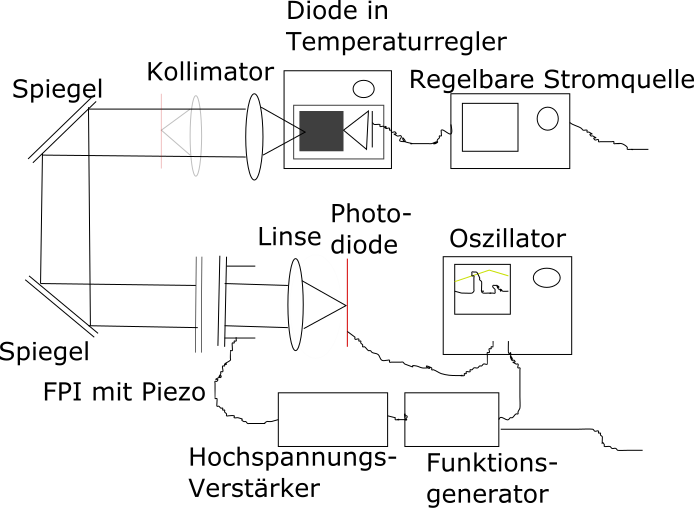
\includegraphics[width= 0.9\textwidth]{Bilder/Aufbau.png}
\caption{Aufbau des Versuches. Die Laserdiode erhält einen Strom aus der regelbaren Stromquelle mit Anzeige. Die Temperatur an der Diode wird durch einen externen Lüfter zwischen 20 und $30^\circ{\text{C}}$ eingestellt. Das von der Diode ausgehende Licht wird mit einer Linse (Kollimator) kollimiert. Im ersten Teil des Versuchs (leicht gezeichnet) wird das Licht danach mit einer Linse auf die Photodiode fokussiert und die Leistung an der Photodiode mit einem Powermeter gemessen. Im zweiten Teil wird das Licht auf ein Fabry-Perot-Interferometer (FPI) gelenkt. Die Spiegelabstände im FPI werden mithilfe des angebrachten Piezo verändert. Der Piezo wird mit einem Hochspannungsverstärker und einem Signalgenerator betrieben. Das vom FPI ausgehende Licht wird mit einer Linse auf eine Photodiode gebündelt. Das Signal der Photodiode und des Funktionsgenerators sind an einem Oszillator sichtbar.
}
\label{fig:Aufbau}
\end{figure}


\section{Leistungscharakteristik}
\label{sec:Leistungscharakteristik}

\subsection{Durchführung}
\label{subsec:Leistung_Durchfuehrung}
Das Experiment wird wie im vorigen Kapitel für den ersten Teil des Experiments aufgebaut sodass man das Licht der Diode ohne weitere Resonatoren mithilfe eines Powermeters und einer Photodiode messen kann. Auf dem an der Phtodiode angeschlossenen Oszillator ist ein Hintergrundsignal mit Frequenz 100 Hz erkennbar. es wird als Umgebungslicht im Labor ermittelt. Der erste Teil des Experiments wird deshalb unter einem Karton gemessen, sodass das Hintergrundrauschen minimiert wird. Es wird die Ausgangsleistung der Diode bei vier verschiedenen Temperaturen mit verschiedenen Stromstärken an der Diode gemessen.

\subsection{Ergebnisse}
\label{subsec:Leistung_Ergebnisse}

\begin{figure}
\centering
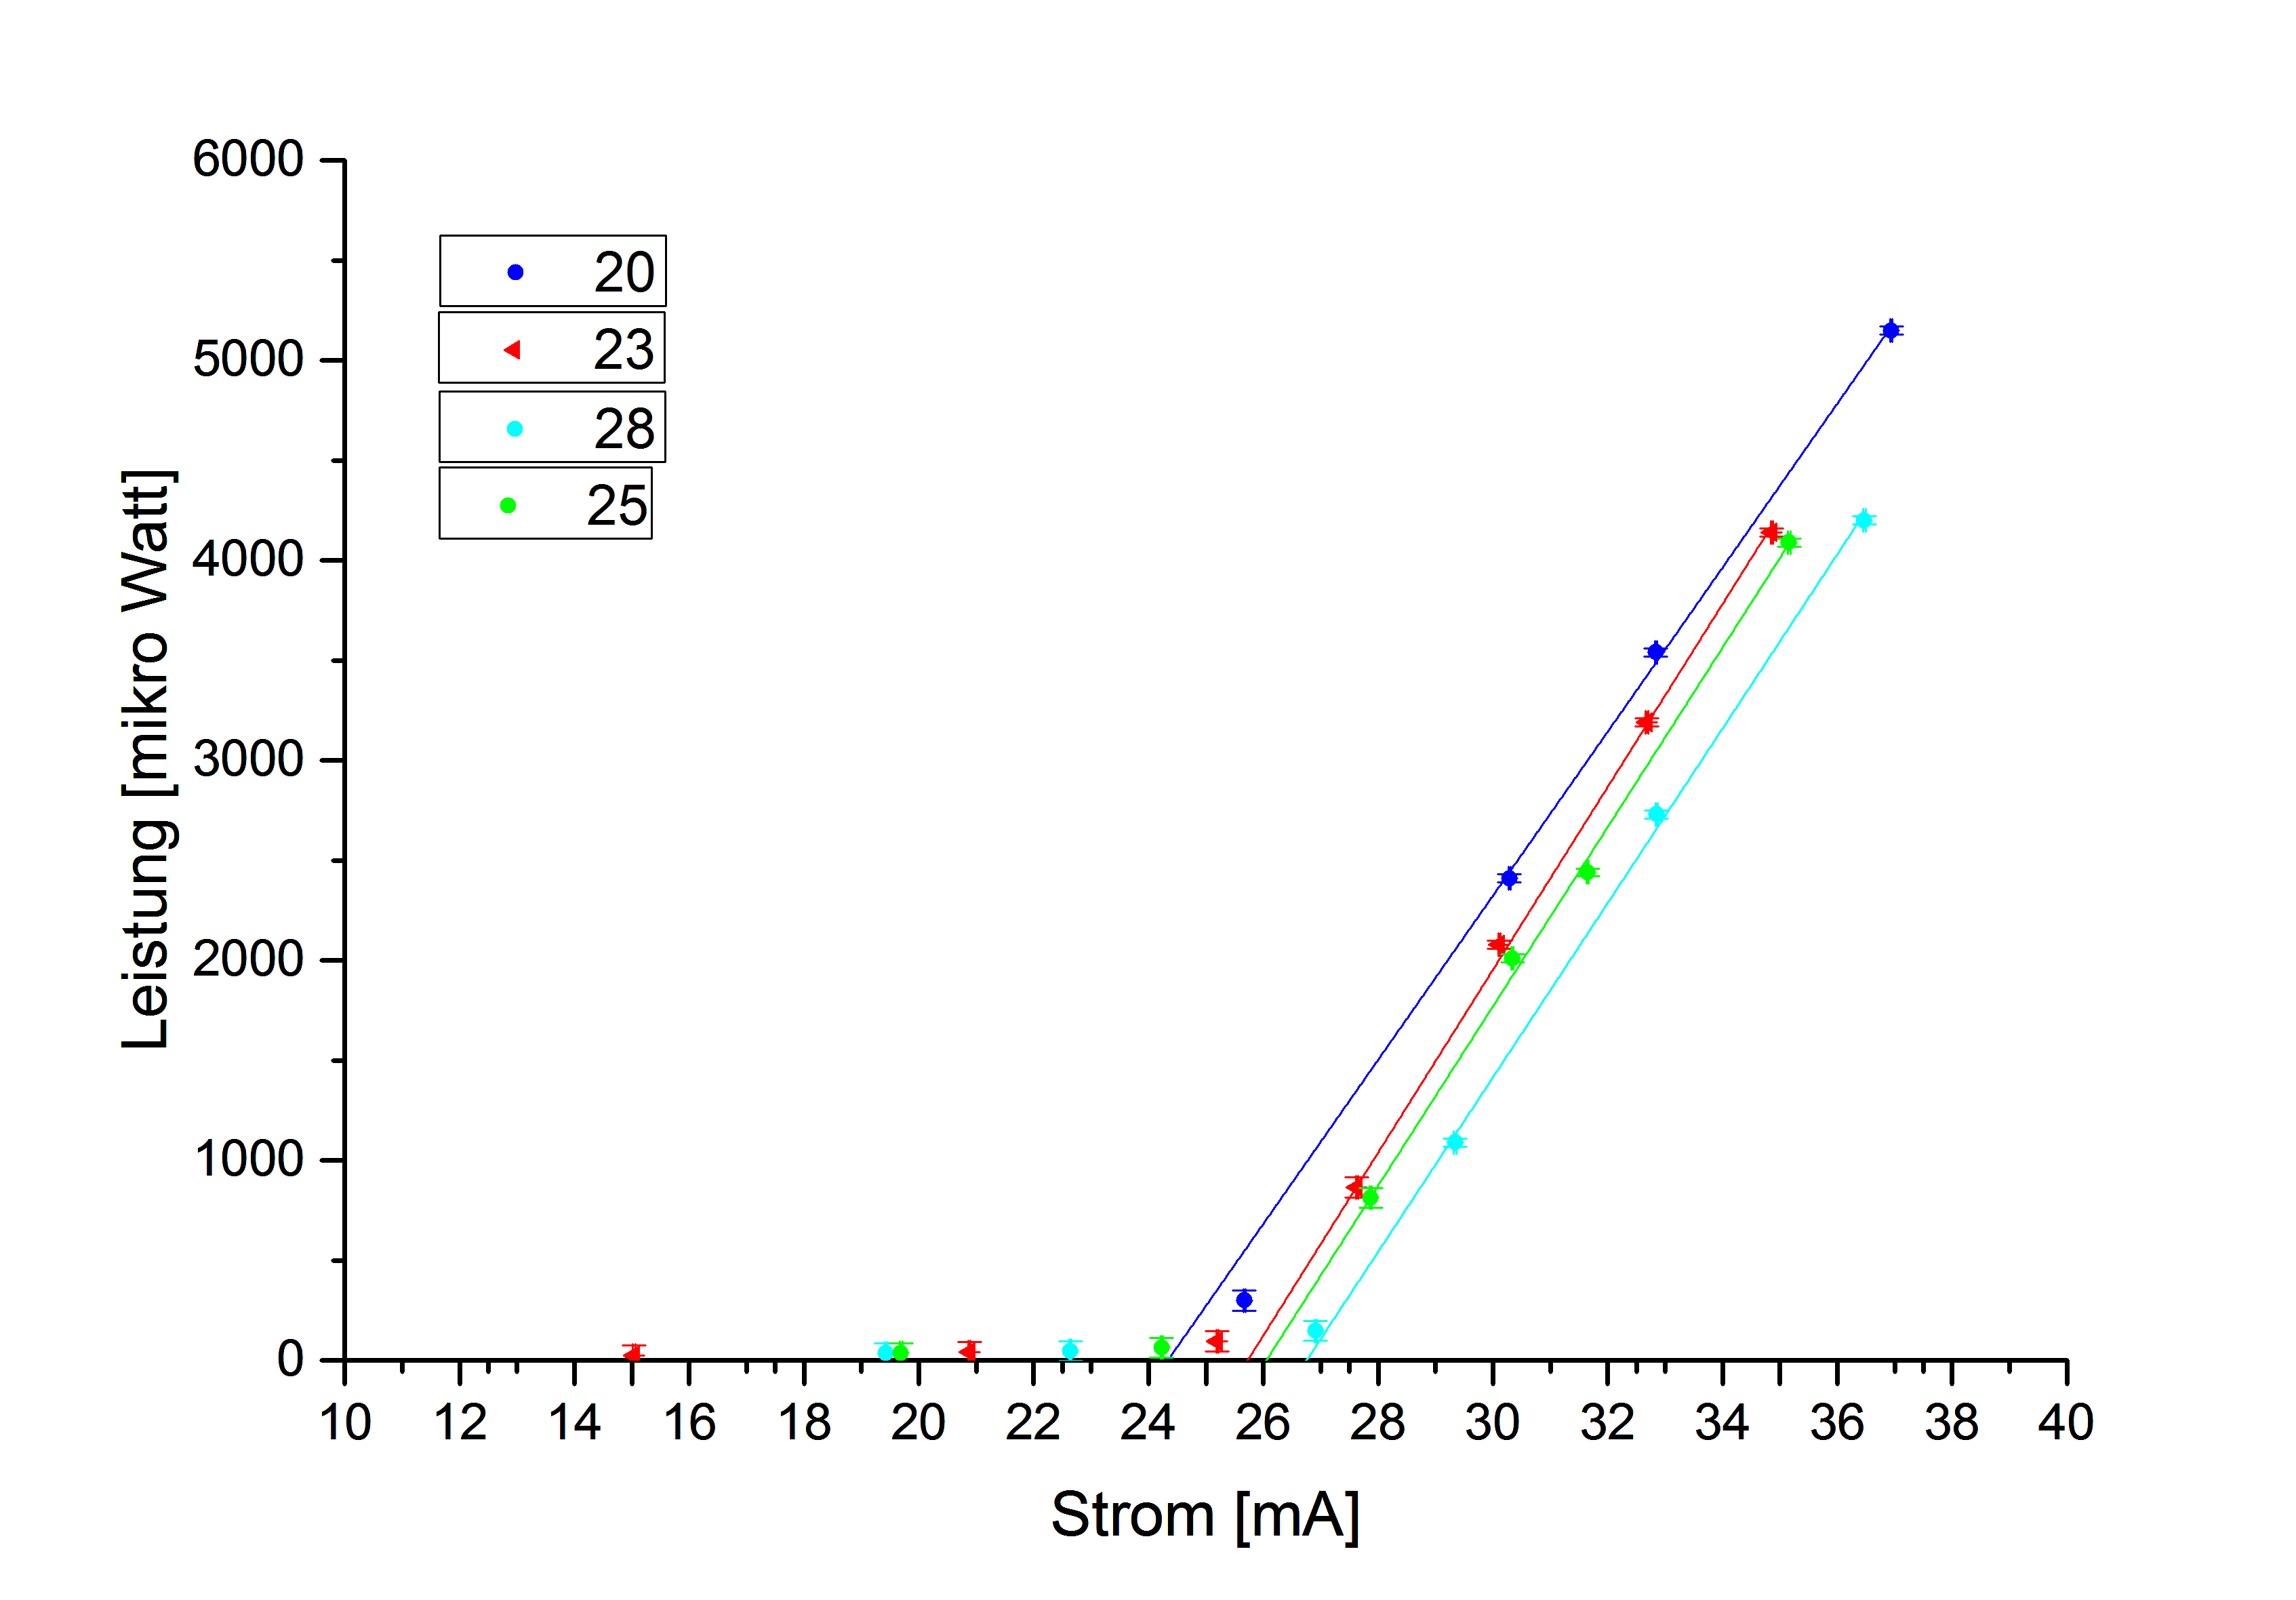
\includegraphics[width=0.8\textwidth]{Bilder/merged_1.png}
\caption{
Gemessene Leistung des Lasers in Abhängigkeit des Diodenstroms bei verschiedenen Temperaturen (in der Legende angegeben, in $^\circ{\text{C}}$). Der Bereich, in dem die Leistung linear ansteigt wurde mit einer linearen Funktion gefittet. Der Schnittpunkt des Fits mit der $x$-Achse beschreibt den Schwellenstrom $I_{\text{th}}$(T) ab dem das Material $lasert$. Die Steigung des linearen Fits beschreibt den Wirkungsgrad $\eta$ der Diode.
}
\label{fig:1_fits}
\end{figure}
Der Fehler beim Ablesen bzw. Einstellen der Temperatur wurde mit $0.1$ $^\circ{\text{C}}$ abgeschätzt. Der Fehler des Kühlers aus [\cite{Mount}] mit $0.02$ $^\circ{\text{C}}$ ist dabei vernachlässigbar. Für die Leistung und Stromstärke wurden Ablesefehler von $0.02$ W und $0.02$ A abgeschätzt.
In Abbildung [\ref{fig:1_fits}] sind die Messwerte aus dem ersten Teil des Versuches dargestellt. Aus den linearen Fits ergibt sich für jede Temperatur ein Schwellenstrom $I_{\text{th}}$, ab dem das Material \emph{lasert} und der Wirkungsgrad $\eta$ der Diode. Aus dem jeweiligen Fit (einzelne Bilder mit Daten des Fits im Anhang) lassen sich $k$ und $y_0$, sowie deren Standardfehler ablesen. Da die Leistung auf der $y$-Achse aufgetragen ist und der Strom auf der $x$-Achse, kann man den Wirkungsgrad $\eta$ mit der Steigung $k$ identifizieren. Der Schwellenstrom entspricht im linearen Fit $y(x) = k\cdot x + y_0$ einem Wert $x_0$ bei dem gilt $y(x_0) = 0$. Es ergibt sich mit Gauss Fehlerfortpflanzung:
\begin{equation}
x_0 = -\frac{y_0}{k}
\end{equation}

\begin{equation}
\Delta x_0 = \sqrt{\left(\frac{\Delta y_0}{k}\right)^2 + \left(\frac{y_0}{k}\Delta k \right)^2}.
\end{equation}

\begin{table}
\centering
\begin{tabular}{||c|c|c|c||}
Temperatur & Schwellenstrom $I_{\text{th}}$ & Wirkungsgrad $\eta$ & Quantenwirkungsgrad $\eta_{\text{Q}}$\\
$[ ^\circ{\text{C}}]$ & [A]	& [W/A] & [ ]\\
\hline
23.0(1)	& 0.0257(6) & 0.457(7) & 0.497(8)\\
25.0(1) & 0.0261(8) & 0.448(9) & 0.49(1)\\
28.0(1) & 0.027(2) &  0.44(2) & 0.48(2)\\
\end{tabular}
\caption{Wirkungsgrad $\eta$, Quantenwirkungsgrad und Schwellenstrom $I_{\text{th}}$ bei verschiedenen Temperaturen. Die Werte und deren Fehler werden aus den Fits des linearen Bereiches der Leistung der Diode in Abhängigkeit des Diodenstromes bestimmt. In Abbildung [\ref{fig:1_fits}] sind diese Fits dargestellt.}
\label{tab:1}
\end{table}

\begin{figure}
\centering
\caption{Die Leistung einer Photodiode bei verschiedenen Temperaturen.}
\label{fig:1_Leistung}
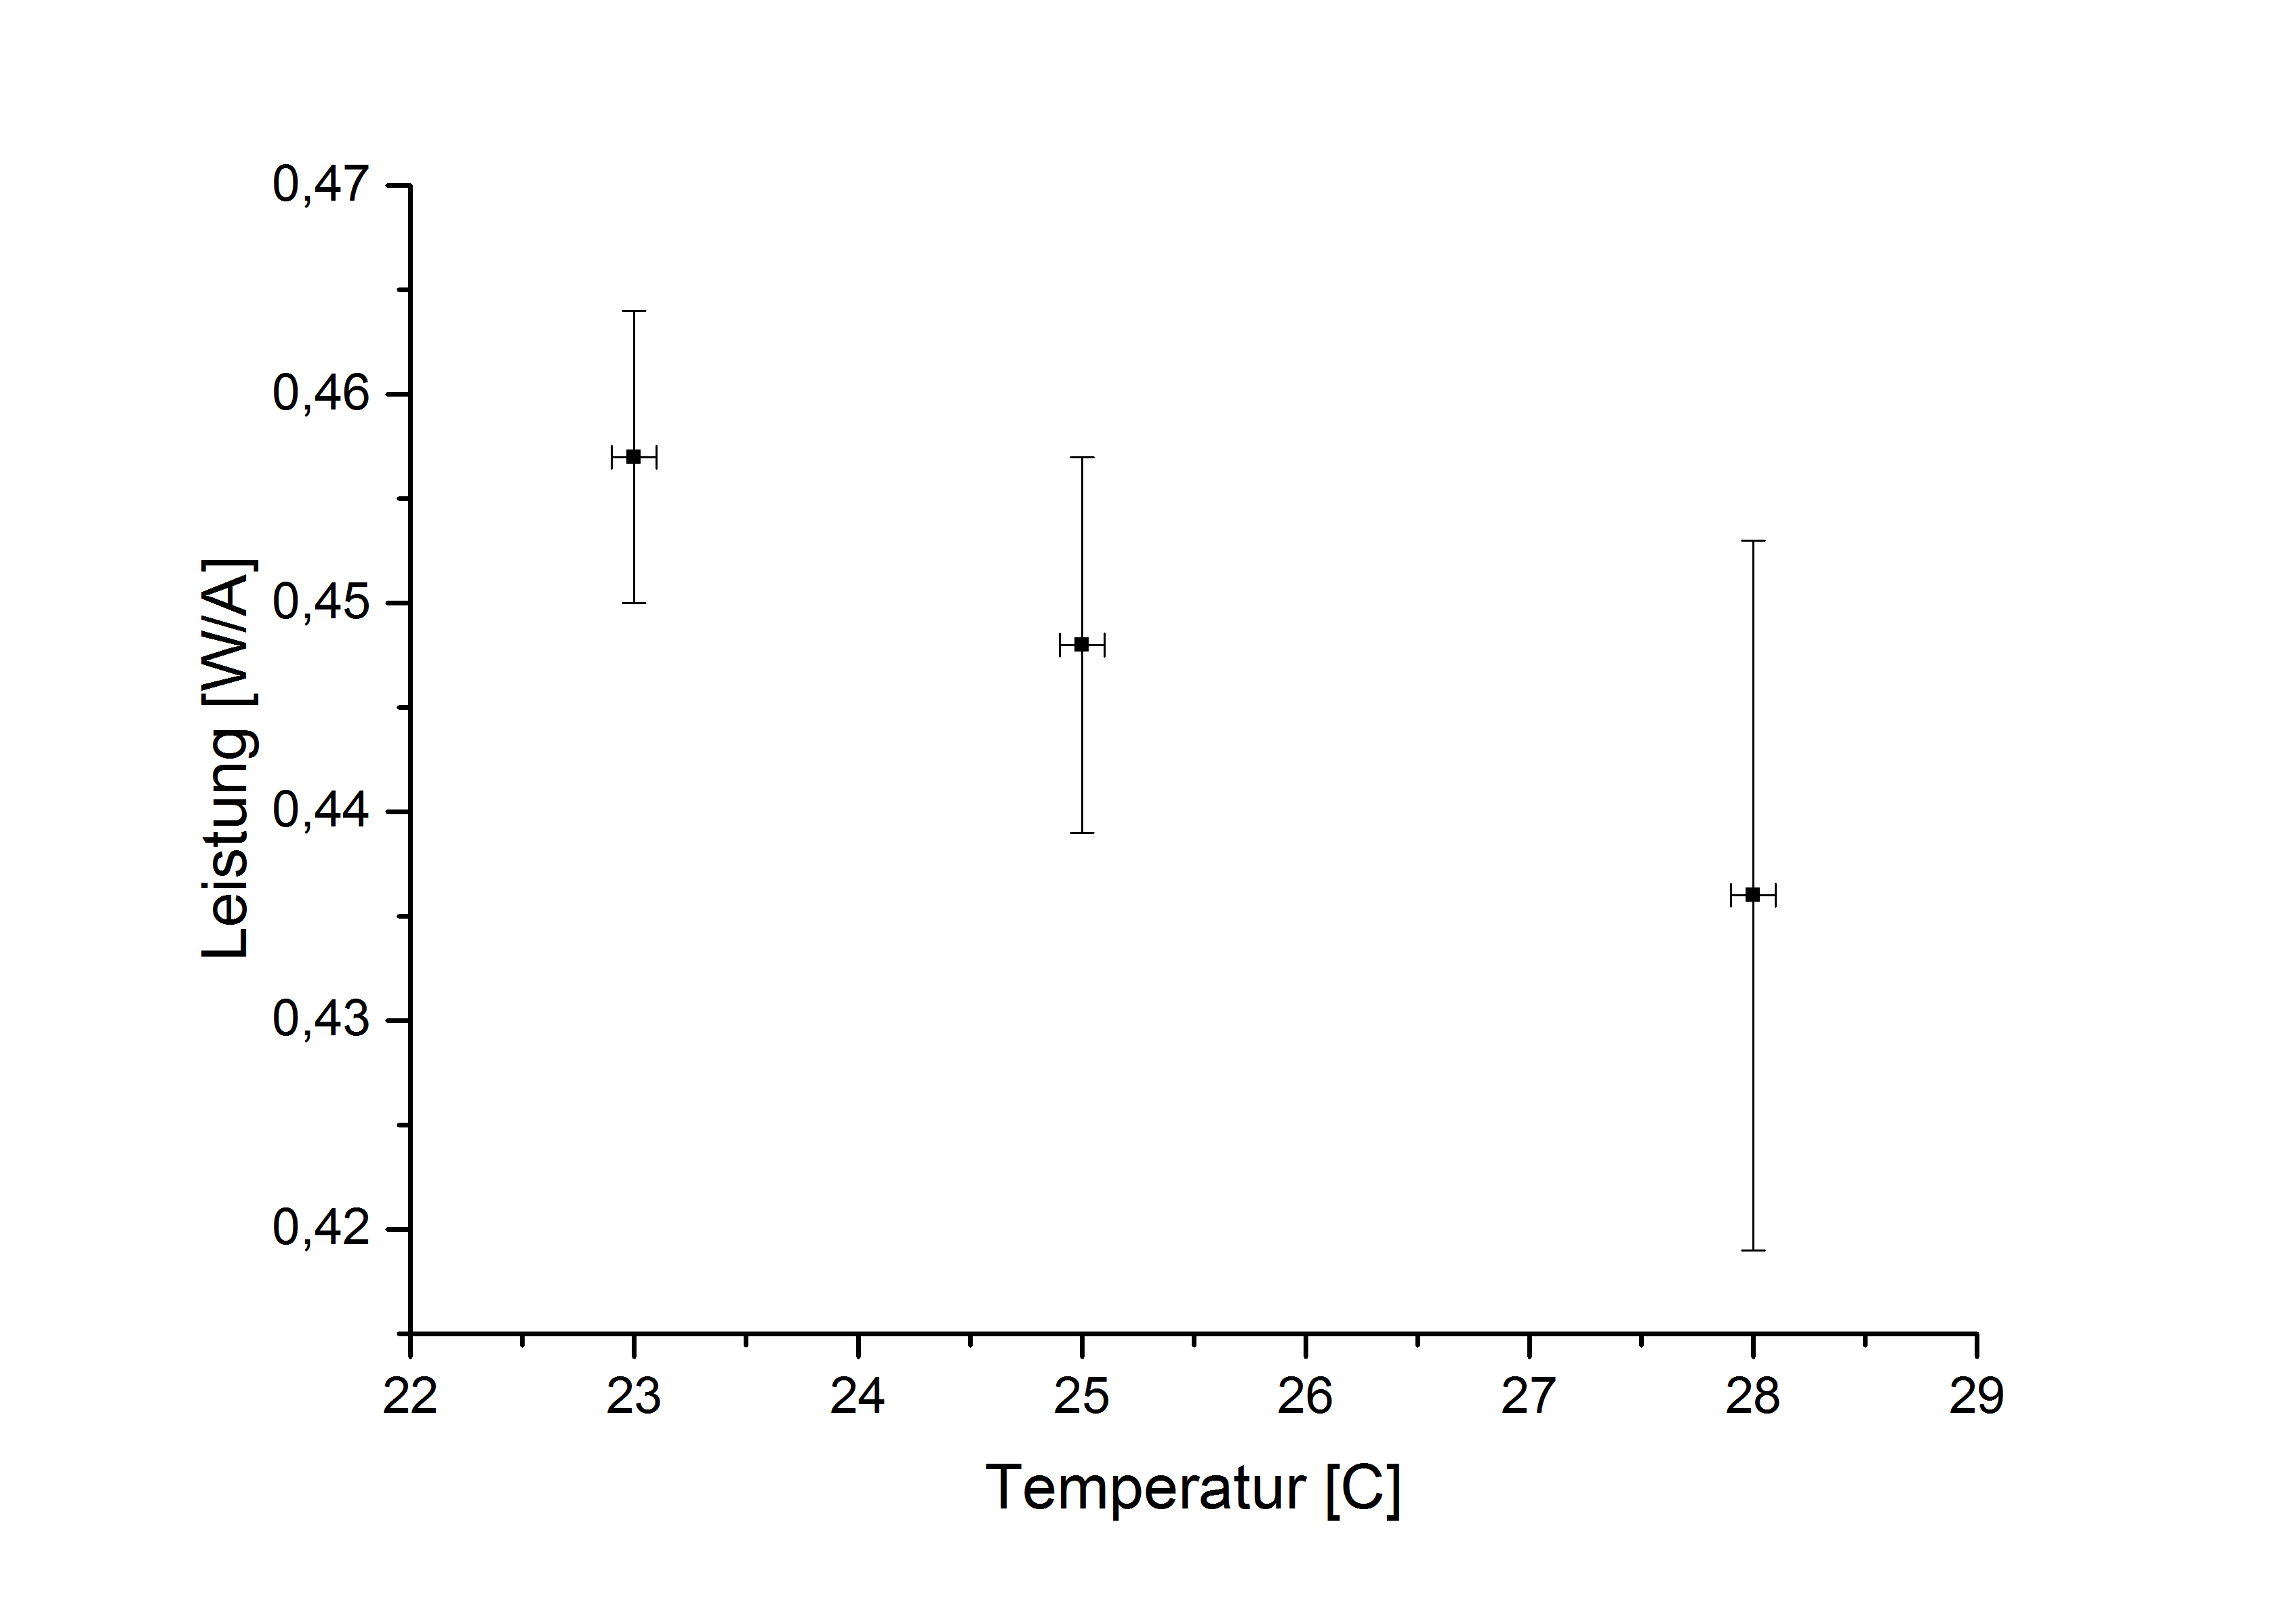
\includegraphics[width=0.8\textwidth]{Bilder/1_Leistung.png}
\end{figure}
\begin{figure}
\centering
\caption{Die Schwellenstrom, ab dem die Photodiode lasert, bei verschiedenen Temperaturen.}
\label{fig:1_Schwellenstrom}
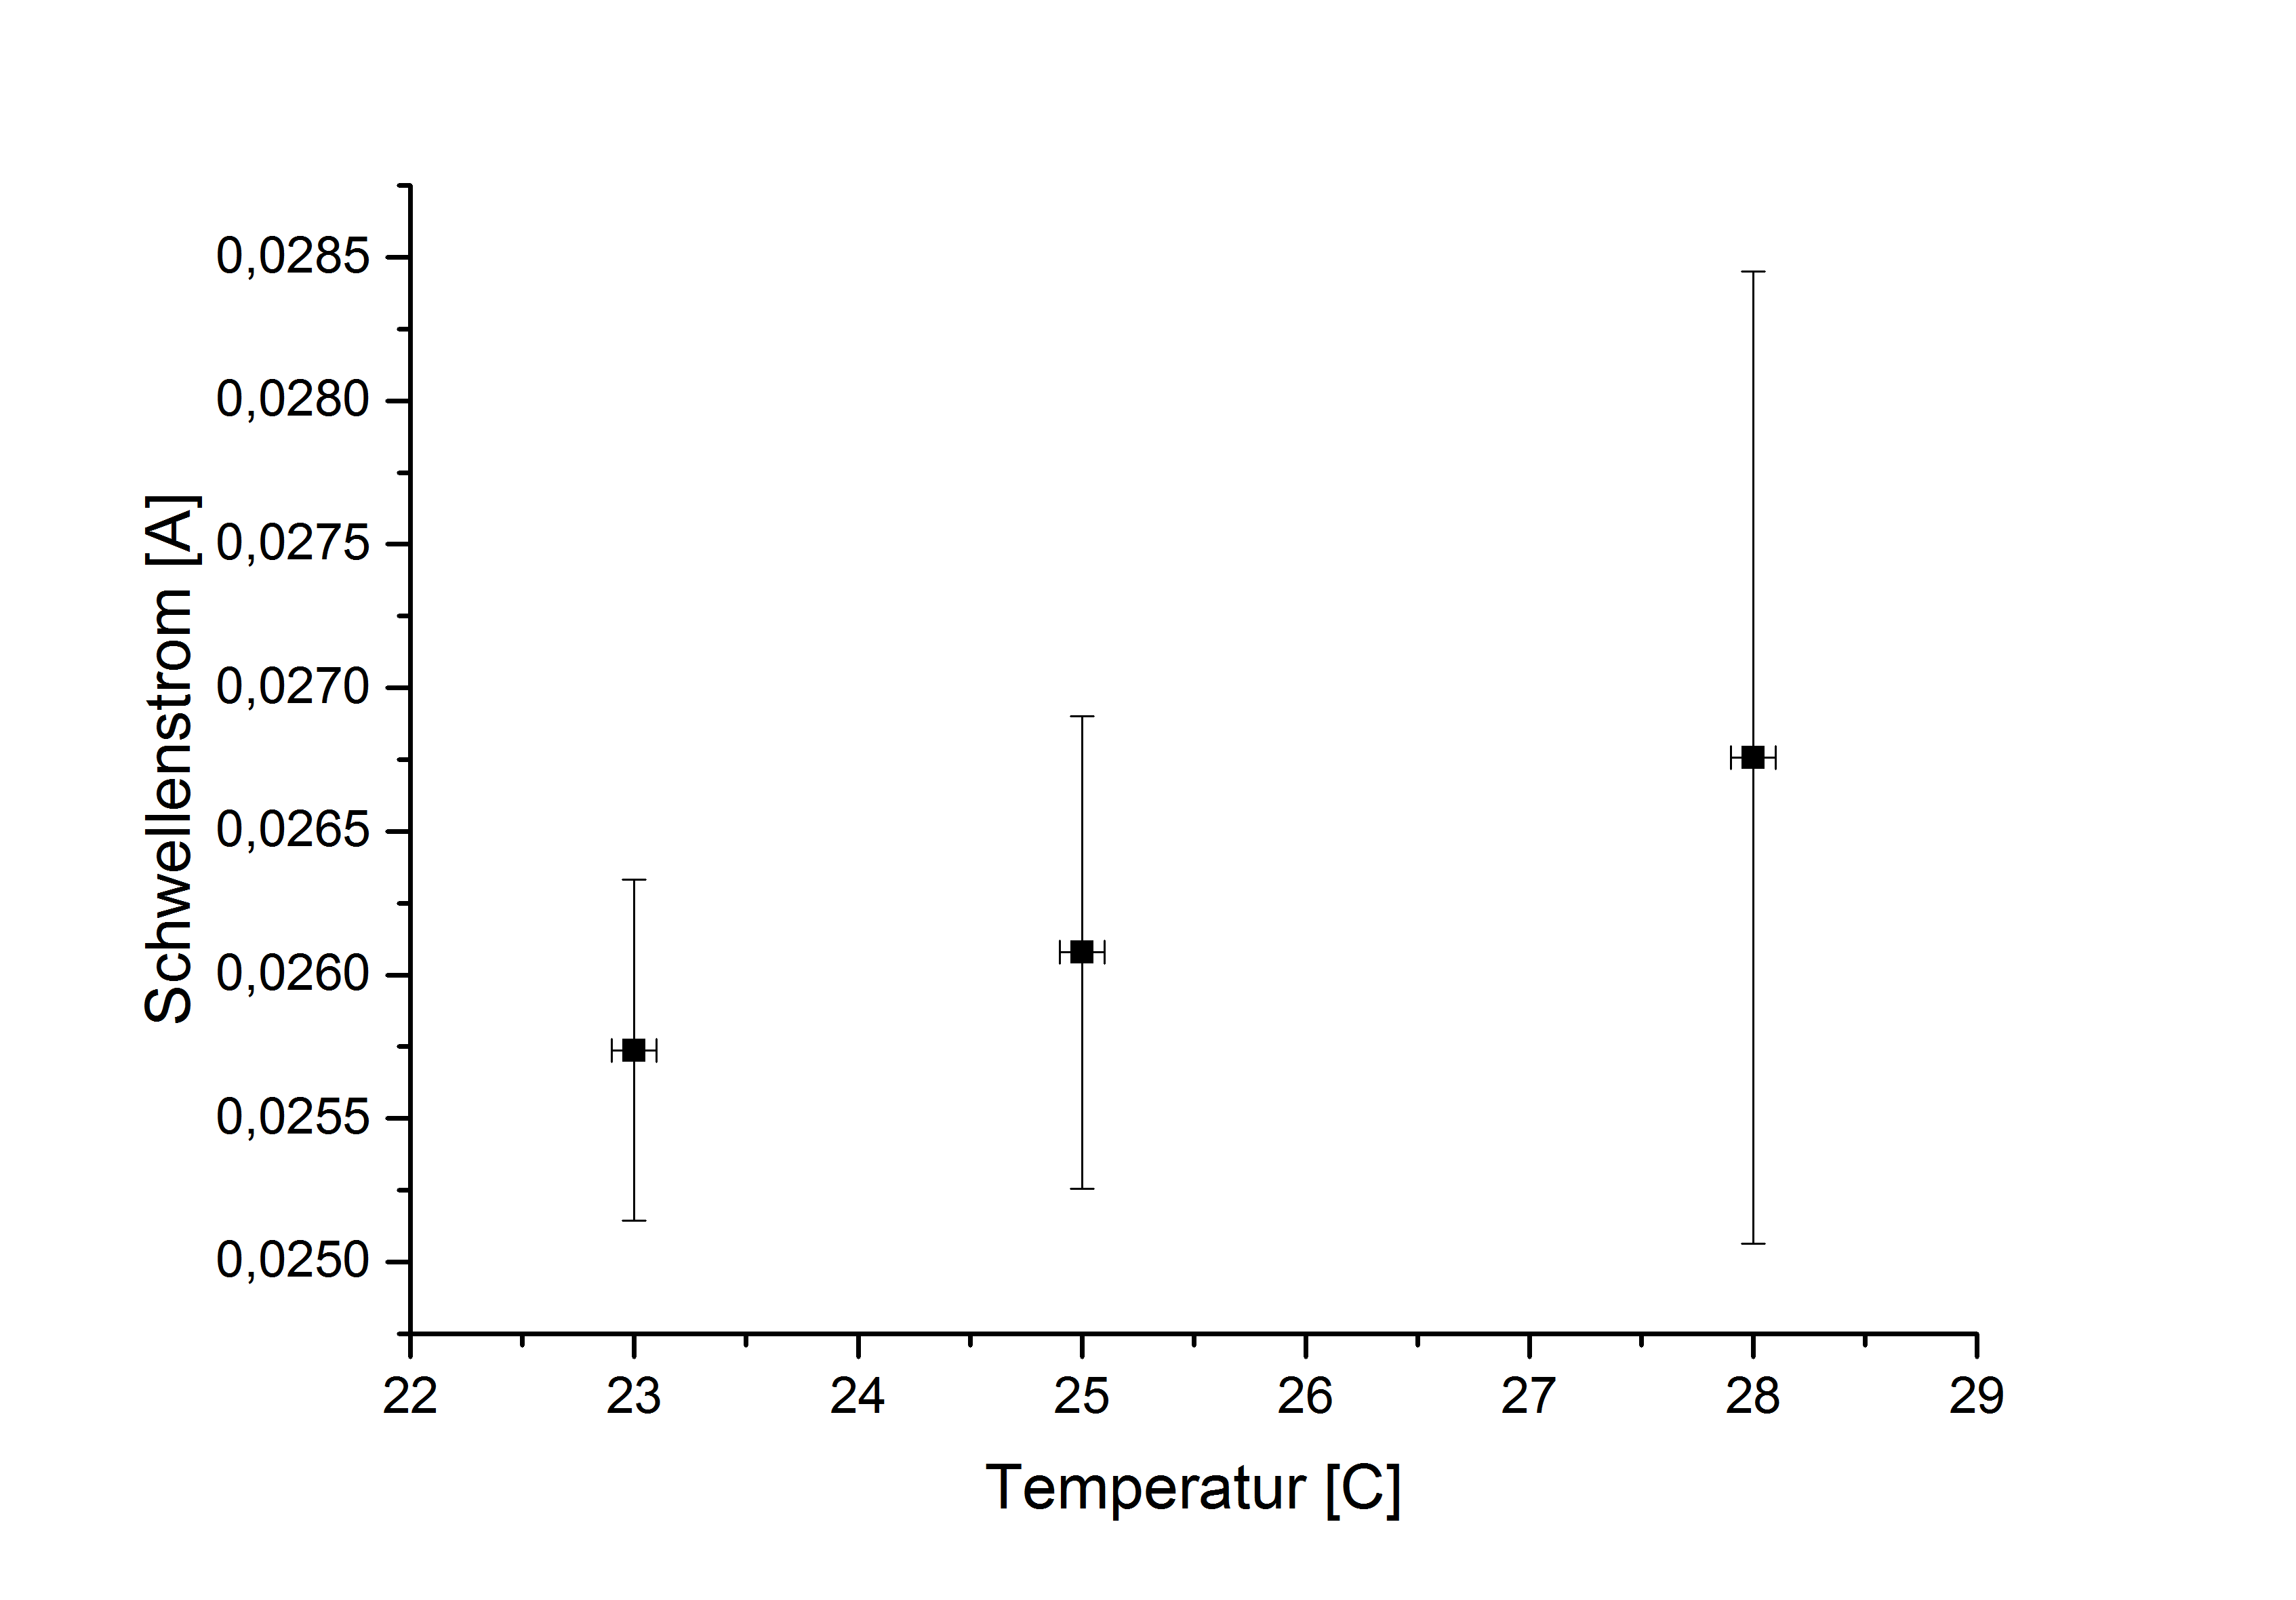
\includegraphics[width=0.8\textwidth]{Bilder/1_Schwellenstrom.png}
\end{figure}
In Abbildung [\ref{fig:1_Leistung}] und Abbildung [\ref{fig:1_Schwellenstrom}] sind die Leistung und der Schwellenstrom, ab dem das Material lasert, bei verschiedenen Temperaturen (Daten aus Tabelle [\ref{tab:1}]) dargestellt.
\subsection{Resume}
\label{subsec_Lesitung_Resume}
Man erkennt, dass der Schwellenstrom mit zunehmender Temperatur (im Bereich $20 - 30 ^\circ{\text{C}}$) steigt und die Leistung abnimmt. In dem Datenblatt zu einer ähnlichen Diode \cite{Diode} wird dies bestätigt.


\section{Frequenzcharakteristik}
\label{sec:Frequenzchar}

\subsection{Durchführung}
\label{subsec:Frequenz_Durchfuehrung}
Das Experiment wird nun wie im Aufbau [\ref{sec:Aufbau}] beschrieben vollständig aufgebaut. Die Photodiode misst dann die Leistung des Lasers nach Durchlaufen eines Fabry-Perot-Resonators. Vor der Messung müssen die beiden Umlenkspiegel so eingestellt werden, dass der Laserstrahl gerade auf das FPI trifft und die zurückreflektierten Strahlen aus dem FPI nicht wieder in die Diode fallen. Weiters müssen die Spiegel des FPI so eingestellt werden, dass man am Ausgang einen möglichst starken Strahl erhält. Die Photodiode und der Funktionsgenerator werden an den Oszillator angeschlossen. Der Funktionsgenerator wird auch mit dem Hochspannungsverstärker, der den Piezo am FPI speisst, verbunden. Es wird eine Dreiecks-Spannung an den Piezo angelegt. Auf dem Oszillator sind die Moden der Diode erkennbar.
\subsection{Ergebnisse}
\label{subsec:Freq_Ergebnisse }
Da die Abmessungen der Diode bekannt sind, ist auch die mittlere freie Weglänge zwischen den Moden der Diode bekannt (150 GHz). Somit kann man mit dem zeitlichen Abstand zwischen zwei Moden auf dem Oszillator den Zeitabstand in einen Frequenzabstand umrechnen. Dies wurde bei konstanter Temperatur und varaiblem Diodenstrom und umgekehrt durchgeführt, um die Frequenzcharakteristik zu erhalten.
\subsubsection{Konstante Temperatur}
Da zwischen der 2. und 4. Mode ein unterschiedlicher Abstand als zwischen zwei benachbarten Moden auftritt, wird angenommen, dass es sich hierbei nicht um einen Modenabstand des Resonators der Diode handelt. Es wird der zweite Datenpunkt bei der Ermittlung des mittleren Abstandes ausgeschlossen, da er sehr stark von den anderen Daten abweicht. Wahrscheinlich handelt es sich dabei um einen Zahlendreher. Dies kann daran liegen, dass das Notieren und Ablesen getrennt werden. Aus den restlichen Daten wird ein mittlerer Modenabstand von $5.08(16)$ ms berechnet, wobei der Fehler der Standardabweichung entspricht. Daraus ergibt sich durch
\begin{align}
\label{eqn:Umrechnung_Time_Freq}
\frac{\Delta \nu}{\Delta t} = \frac{150 \text{GHz}}{5.08 \text{ms}}
\end{align}
die Umrechnung von Sekunden in Hertz. In Abbildung [\ref{fig:2_const_T}] ist die Frequenzcharakteristik bei konstanter Temperatur $T = 22.0(1) $ $^\circ{\text{C}}$ aufgezeichnet.
\begin{figure}
\centering
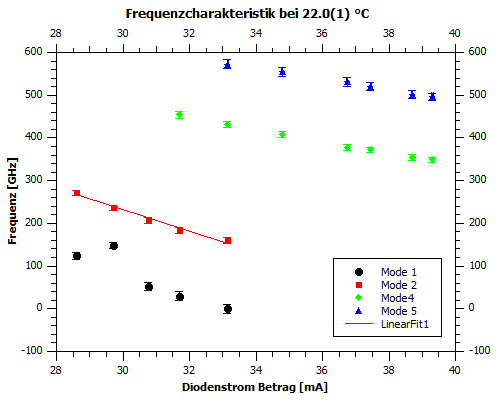
\includegraphics[width=0.8\textwidth]{Bilder/Frequenzchar_1.png}
\caption{Der Verlauf der Moden bei konstanter Temperatur und unterschiedlichem Diodenstrom. Die Abstände der Dioden werden auf einem Oszillator gemessen und mit Gleichung [\ref{eqn:Umrechnung_Time_Freq}] in Frequenzabstände umgerechnet. Der lineare Fit der zweiten Mode ist eingezeichnet.}
\label{fig:2_const_T}
\end{figure}
Die Fehler ergeben sich jeweils aus dem Ablesen der Temperatur, des Diodenstroms, der Zeit, sowie aus dem Umrechnen der Zeit in die Frequenz. Zur Berechnung des gesamten Fehlers wird Gauss Fehlerfortpflanzung verwedet. Die einzelnen Moden (ohne Modensprünge) werden mit einem linearen Fit approximiert. Aus den linearen Fits aller Moden ergibt sich ein Frequnzabfall von $-17(1) \,\frac{\text{GHz}}{\text{mA}}$.

\subsubsection{Konstanter Strom}
Die Frequenzcharakteristik bei konstantem Strom und unterschiedlichen Temperaturen im Bereich zwischen $20 \, \text{und} \, 30 $ $^\circ{\text{C}}$ wird ebenfalls für jeden Messpunkt aus dem Oszillator gelesen und mit Gleichung [\ref{eqn:Umrechnung_Time_Freq}] in einen Frequenzabstand umgerechnet.
\begin{figure}
\centering
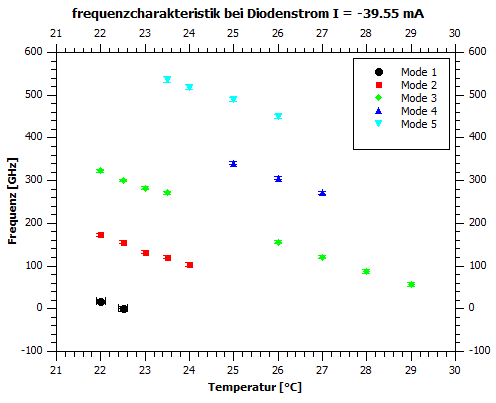
\includegraphics[width=0.8\textwidth]{Bilder/Frequenzchar_2.png}
\caption{Der Verlauf der Moden bei konstantem Strom  und unterschiedlicher Temperatur an der Diode. Die Abstände der Dioden werden auf einem Oszillator gemessen und mit Gleichung [\ref{eqn:Umrechnung_Time_Freq}] in Frequenzabstände umgerechnet.}
\label{fig:2_const_I}
\end{figure}
In Abbildung [\ref{fig:2_const_I}] ist die Frequenzcharakteristik bei konstantem Diodenstrom $I = -39.55(2)$ mA aufgezeichnet.\\
Für steigenden Diodenstrom und steigende Temperatur sinkt die Frequenz. In beiden Abbildungen erkennt man, dass die Moden einen linearen Frequenzabfall verzeichnen, bis sie einen Modensprung durchführen. In den Plots sind die Moden numeriert, sodass das Frequenzverhalten ohne Modensprünge beobachtet werden kann. Wie für die Frequenzcharakteristik bei konstanter Termperatur wird auch für konstanten Diodenstrom die Frequenzcharakteristik berechnet und gibt $-35(2)$ $\frac{\text{GHz}}{\text{K}}$.


\section{Anhang}
\label{sec:Anhang}
\begin{figure}
\caption{Messreihe zum 1. Teil des Versuches bei $23 ^\circ{\text{C}}$. Leistung der Diode in Abhängigkeit des Stromes. Jeweilige Fehler aus dem Ablesen der Messswerte. Die Messwerte werden linear gefittet.}
\label{fig:1_25}
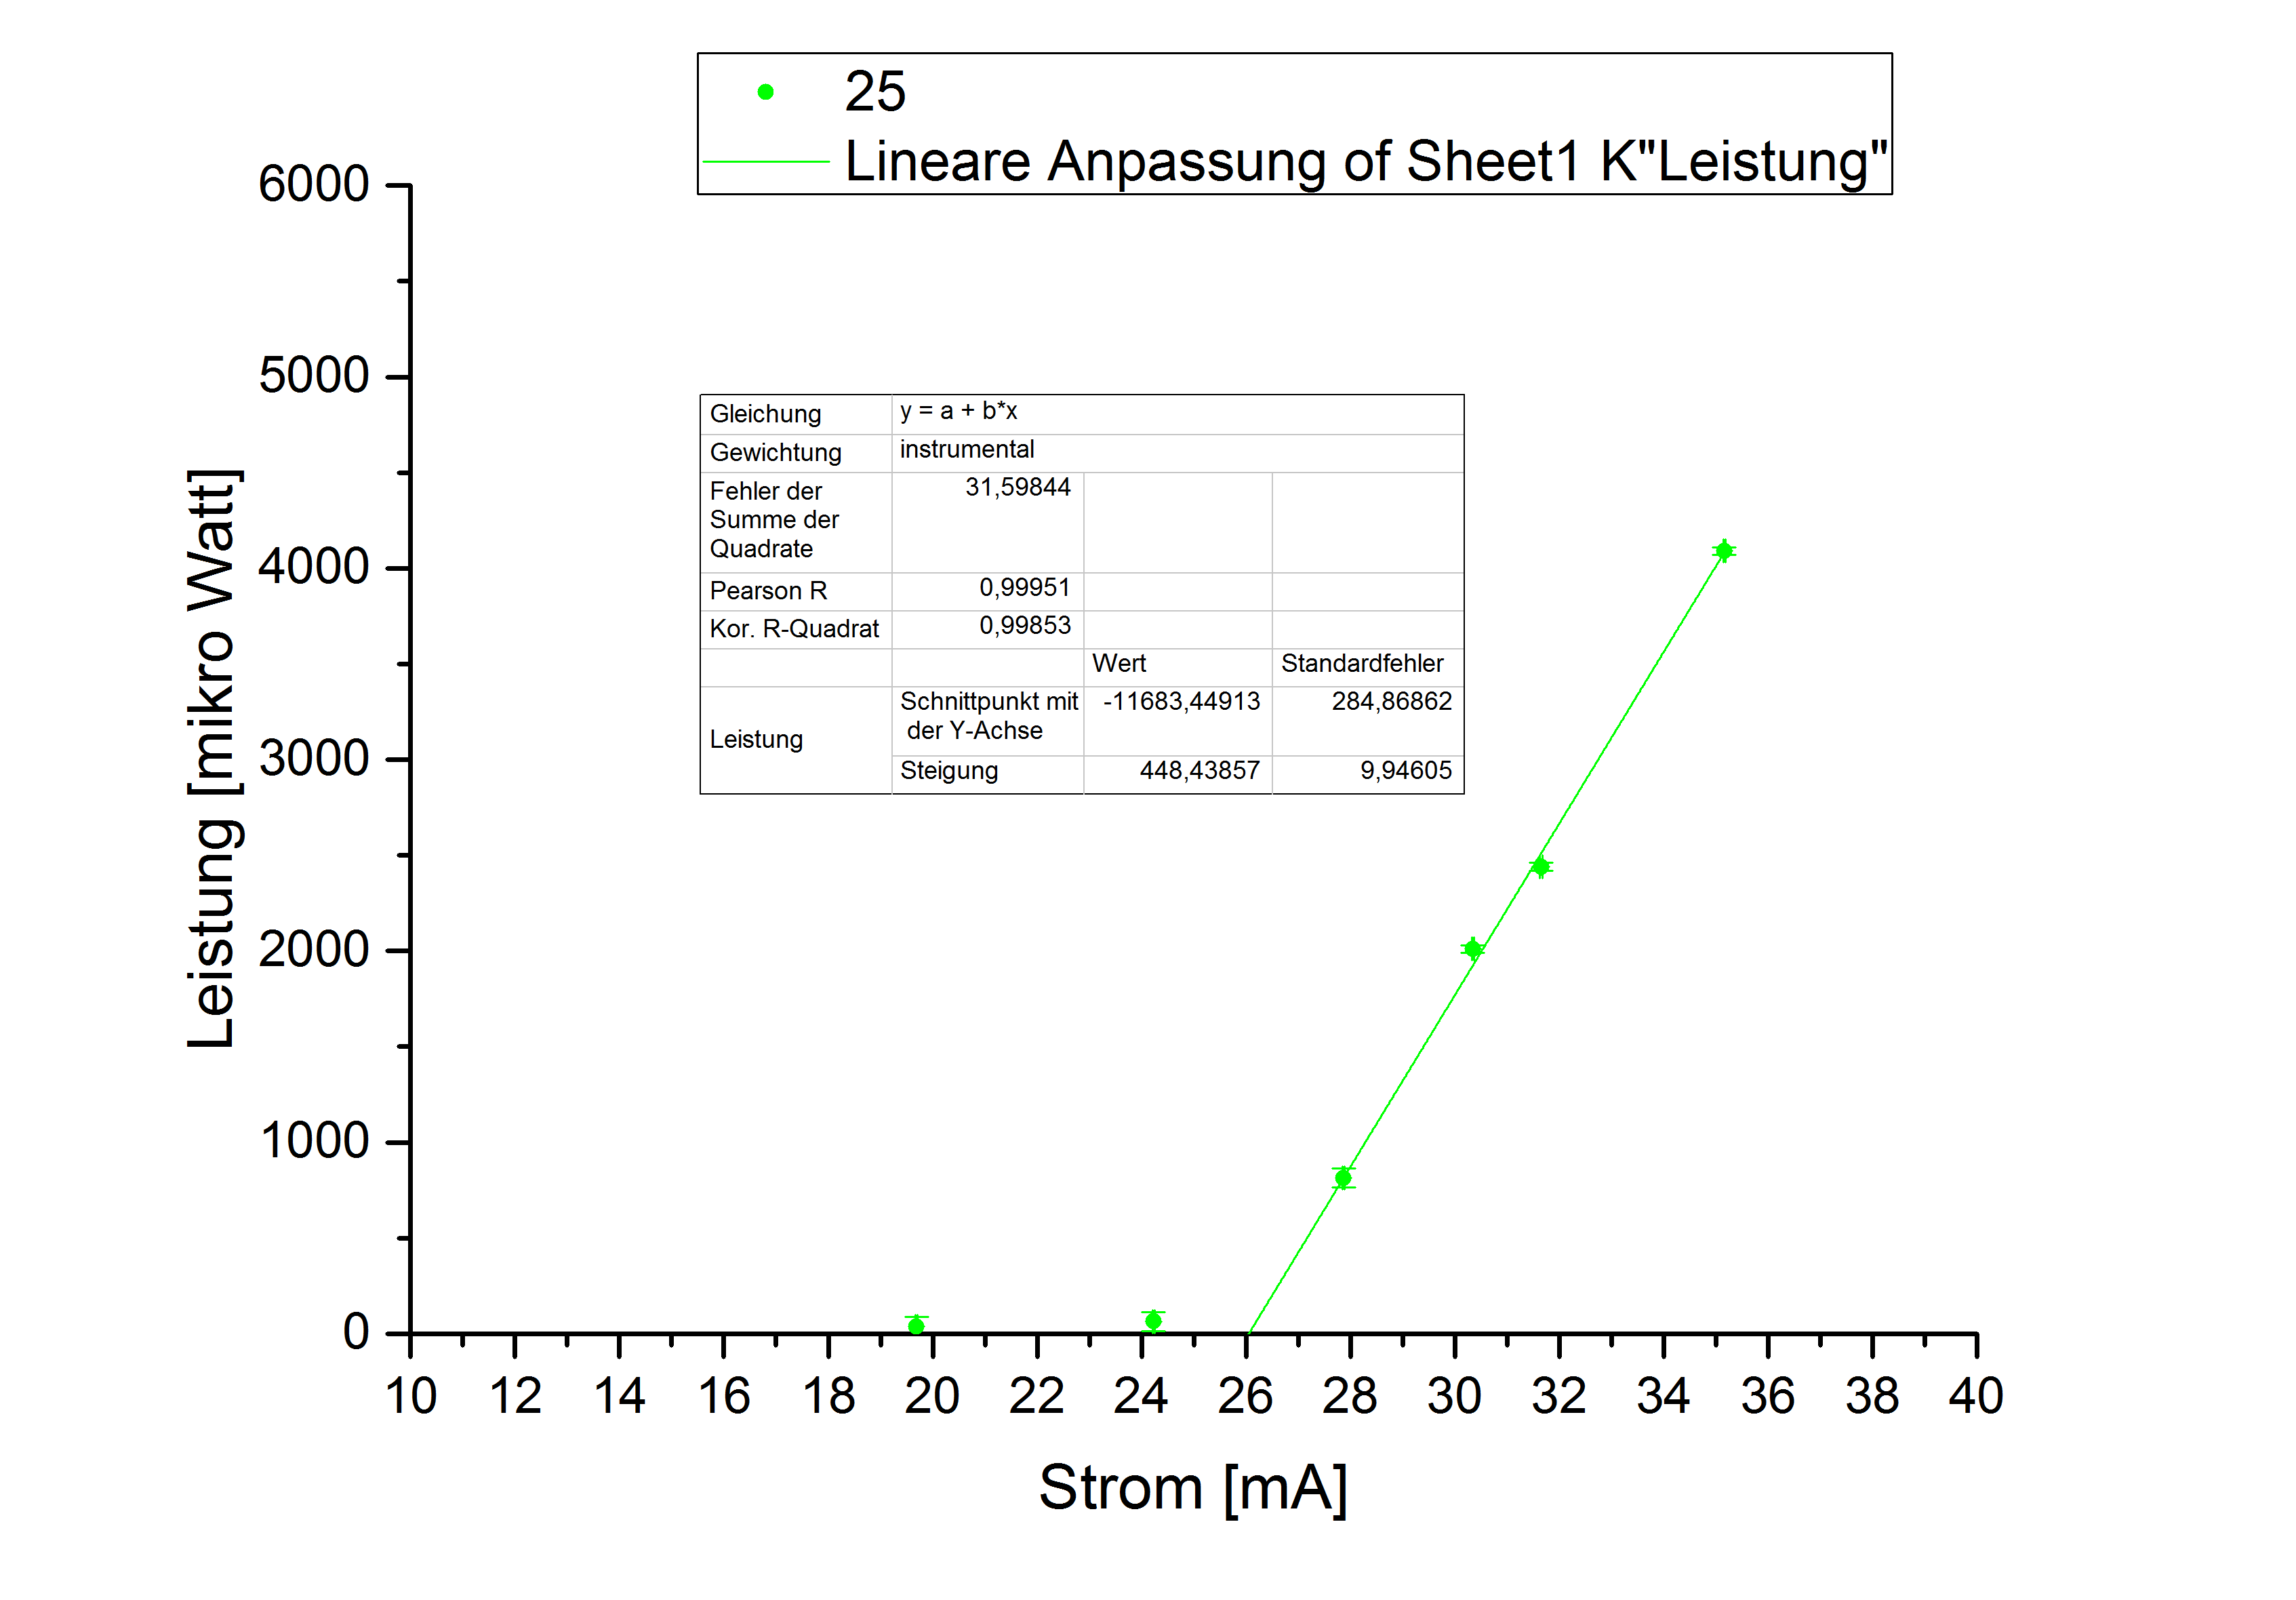
\includegraphics[width = 0.75\textwidth]{Bilder/25.png}
\end{figure}
\begin{figure}
\caption{Messreihe zum 1. Teil des Versuches bei $25 ^\circ{\text{C}}$. Leistung der Diode in Abhängigkeit des Stromes. Jeweilige Fehler aus dem Ablesen der Messswerte. Die Messwerte werden linear gefittet.}
\label{fig:1_28}
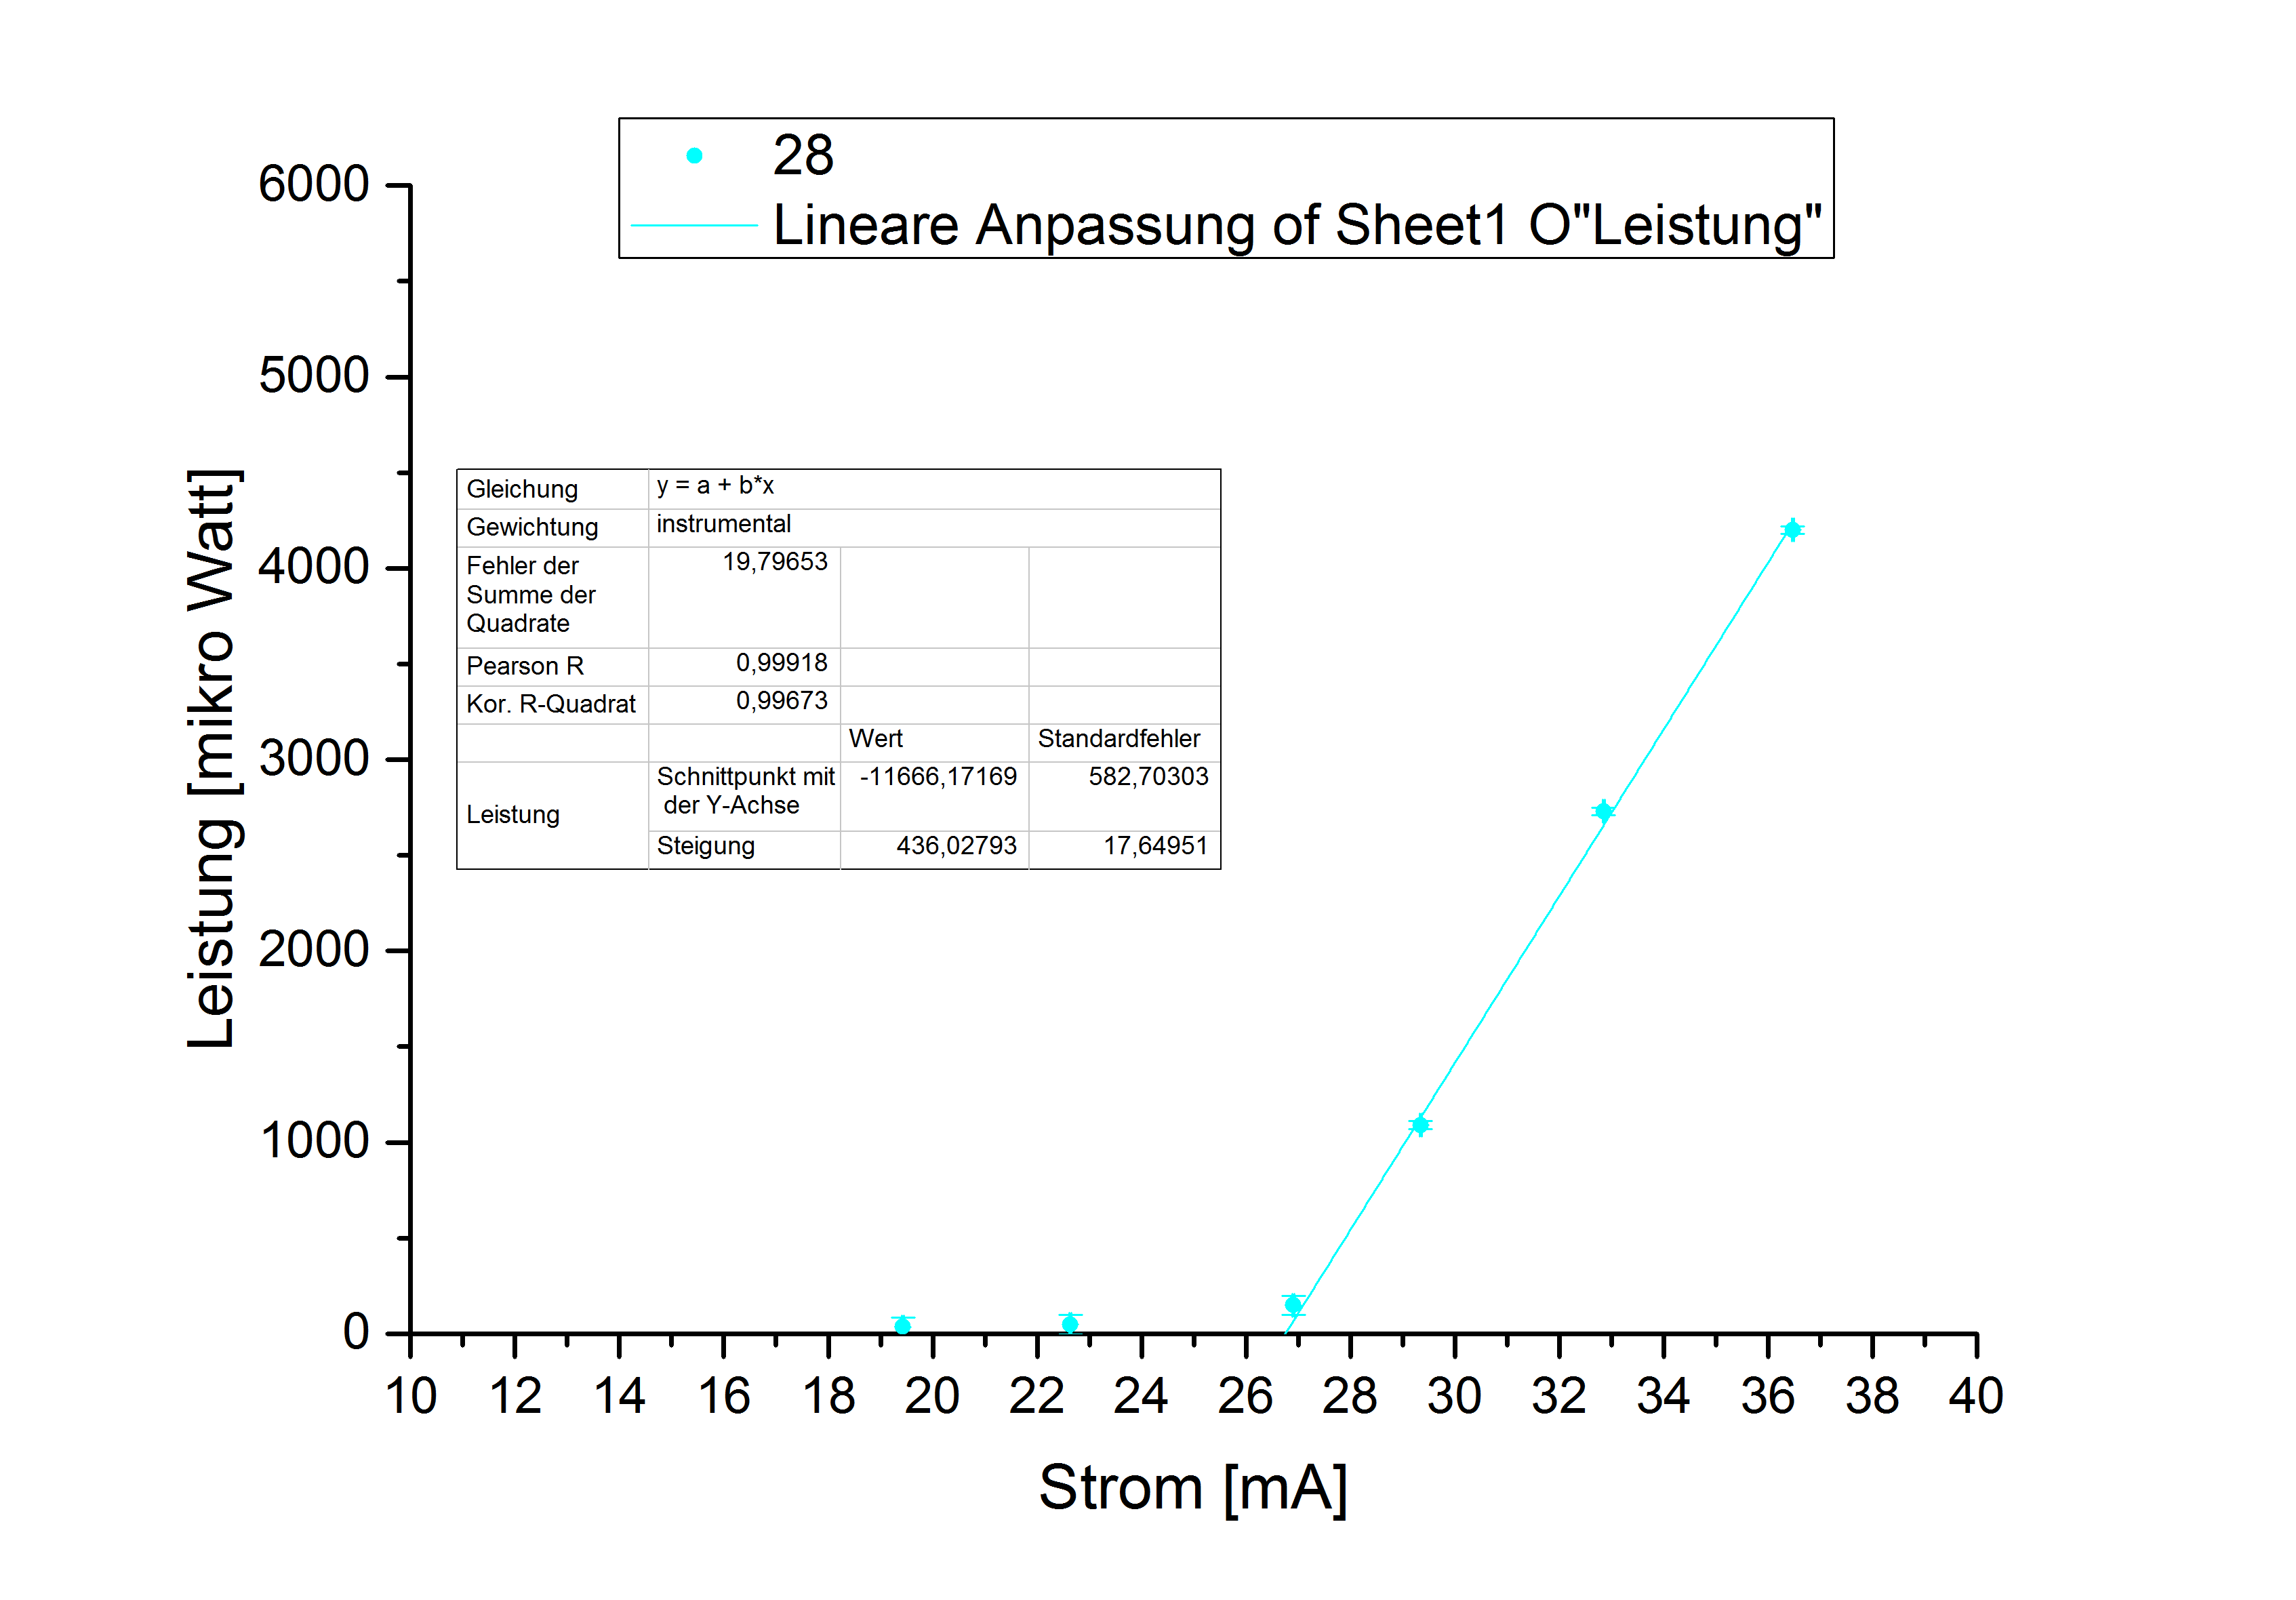
\includegraphics[width = 0.75\textwidth]{Bilder/28.png}
\end{figure}
\begin{figure}
\caption{Messreihe zum 1. Teil des Versuches bei $28 ^\circ{\text{C}}$. Leistung der Diode in Abhängigkeit des Stromes. Jeweilige Fehler aus dem Ablesen der Messswerte. Die Messwerte werden linear gefittet.}
\label{fig:1_23}
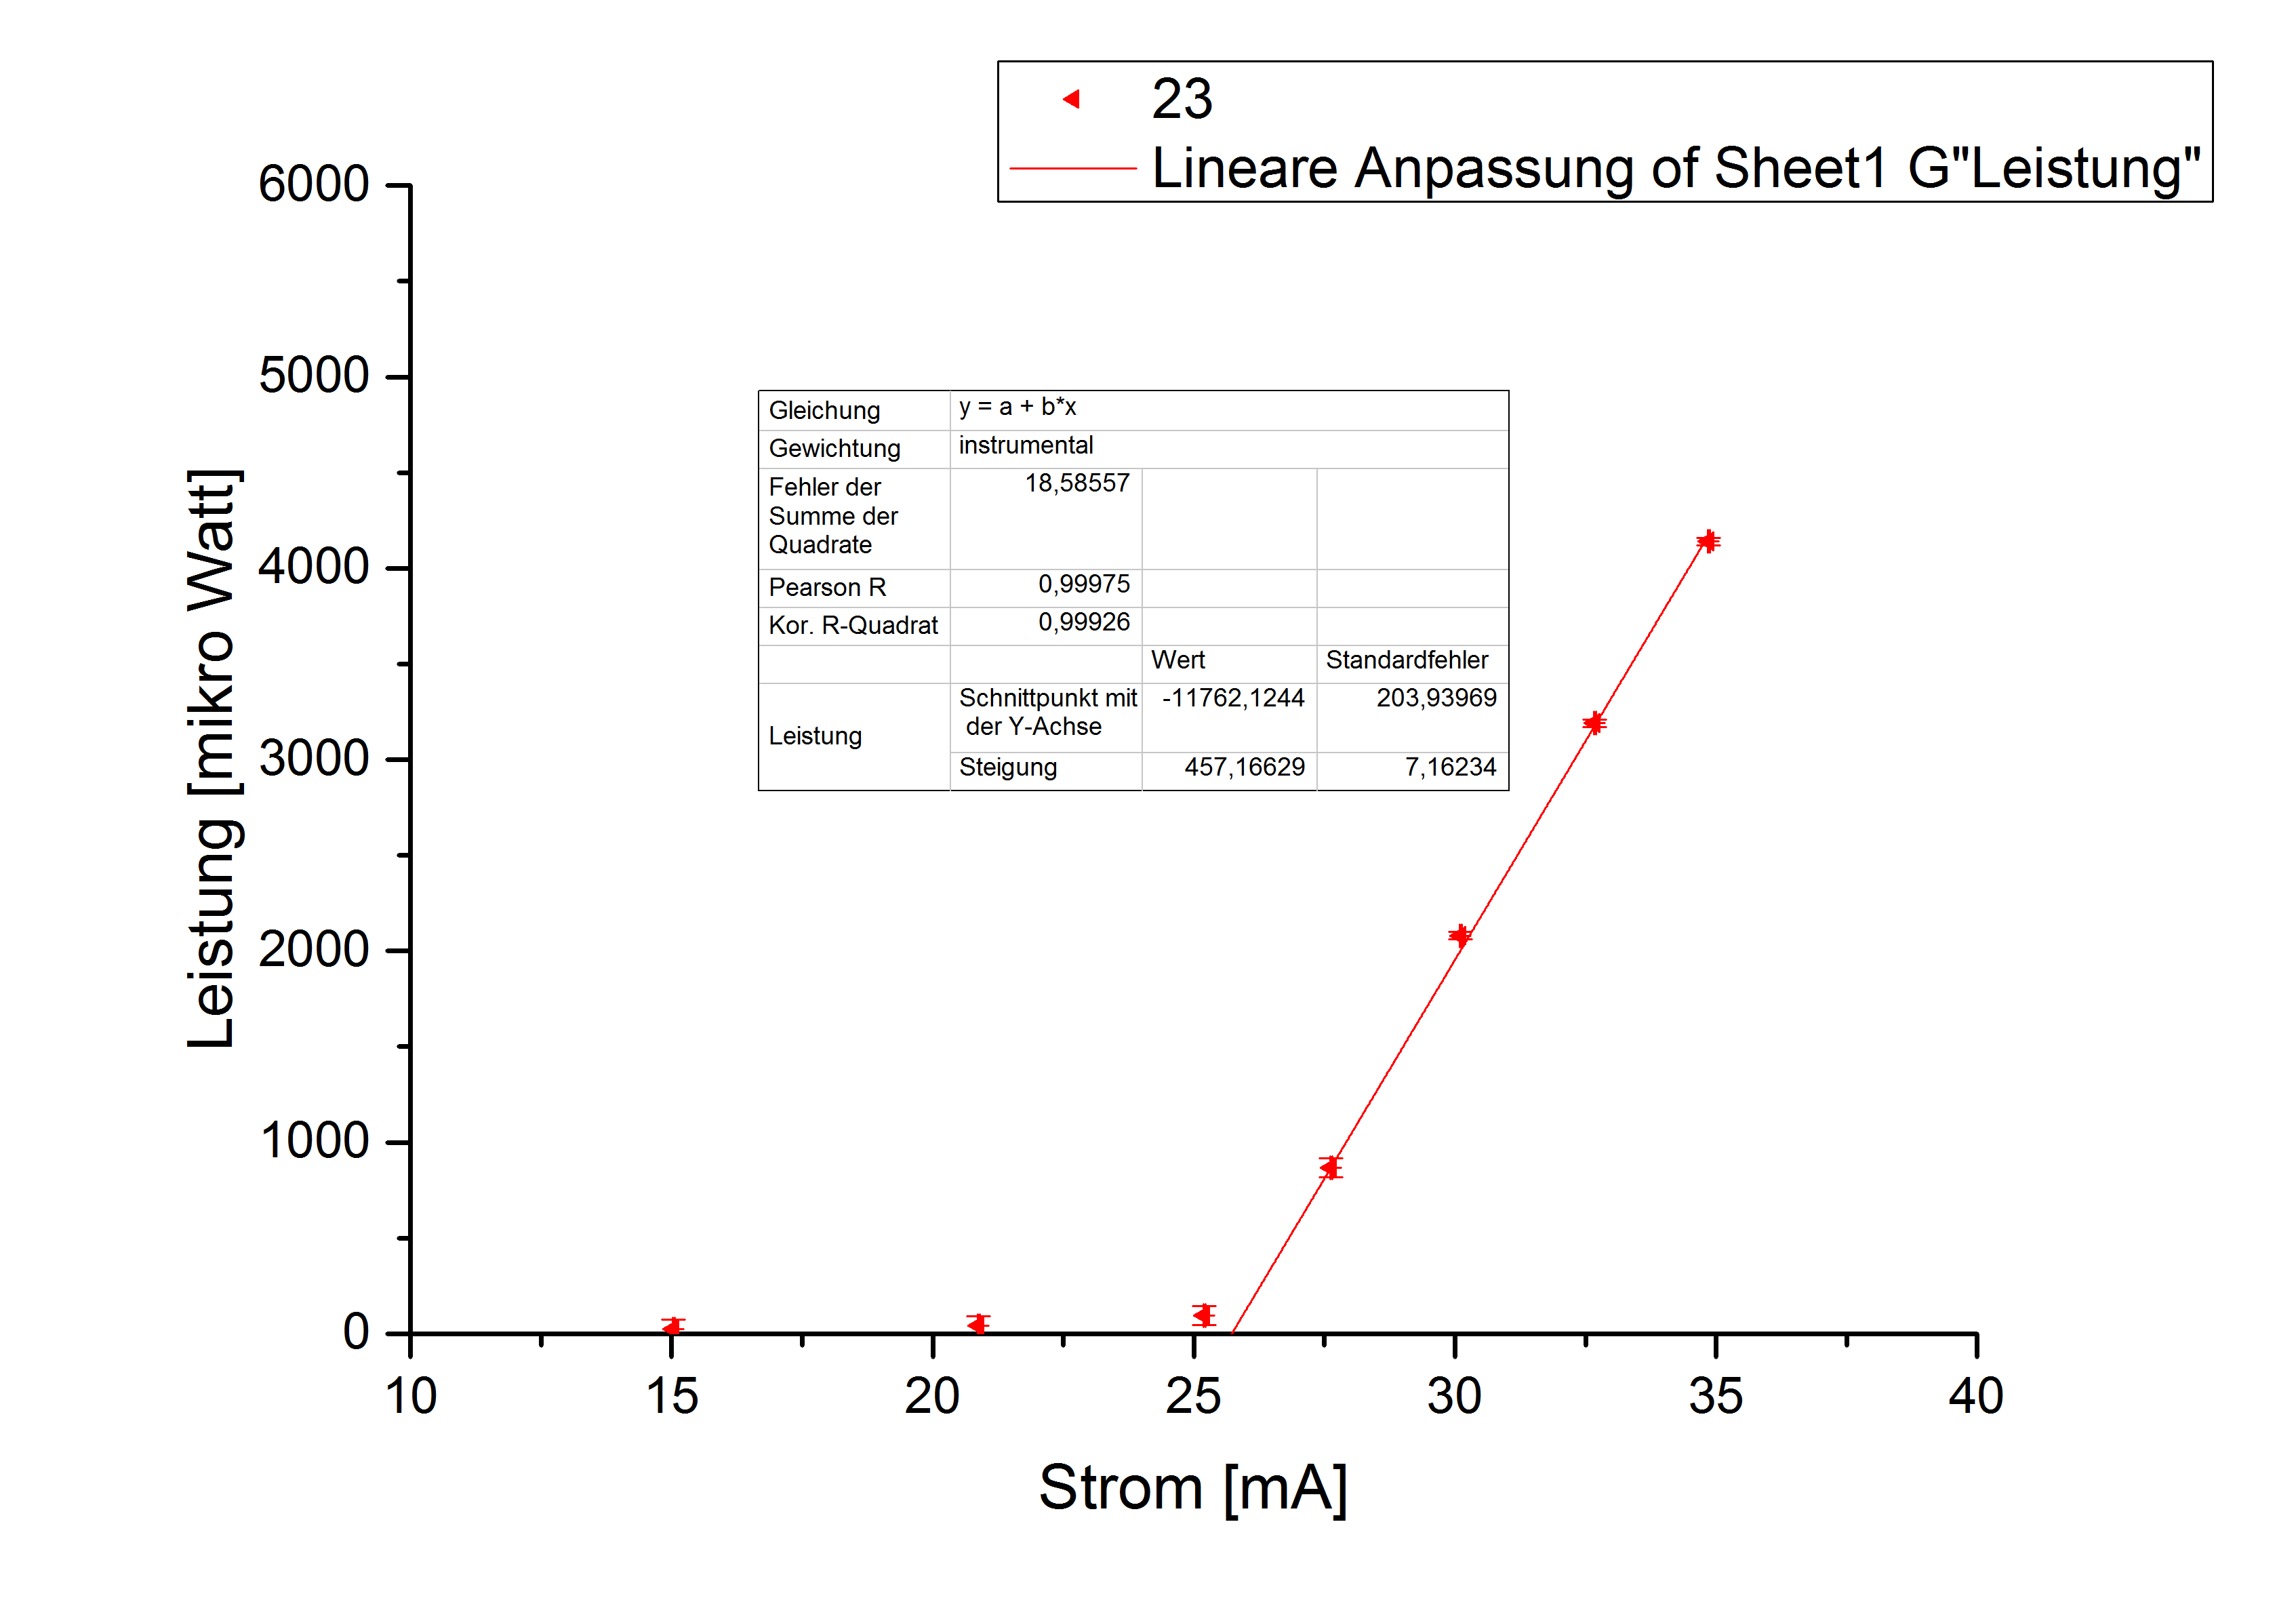
\includegraphics[width = 0.75\textwidth]{Bilder/23.png}
\end{figure}
\begin{thebibliography}{9}
\bibitem{Marx}
Festkörperphysik, R. Gross, A. Marx, De Gruyter

\bibitem{Mount}
\href{https://www.thorlabs.de/newgrouppage9.cfm?objectgroup_id=5583&pn=LDM9T/M}{Thorlabs: Laser Diode Mount with Integrated TEC and Controller}

\bibitem{Diode}
\href{https://lms.uibk.ac.at/auth/1%3A1%3A1052805258%3A2%3A0%3Aserv%3Ax/datasheet_HL6712G.pdf}{Hitachi HL6712G AlGaInP Laser Diode}

\bibitem{Anleitung}
\href{https://lms.uibk.ac.at/auth/1%3A1%3A1050700822%3A2%3A0%3Aserv%3Ax/diode110.pdf}{Anleitung Versuch Diodenlaser, Universität Innsbruck}

\end{thebibliography}

\end{document}